  % table?
  Important heat limits in materials of the repository restrict loading designs 
  and capacity.
  %        File: heat_tab.tex
%     Created: Thu Aug 04 11:00 AM 2011 C
% Last Change: Thu Aug 04 11:00 AM 2011 C
%
\begin{table}[h!]
  \centering
  \footnotesize{
  \begin{tabular}{|l|r|r|r|r|}
    \multicolumn{5}{c}{\textbf{Thermal Behavior of Various Concepts}}\\
    \hline
            & Clay & Granite & Salt & Deep \\ 
            & & & & Borehole \\ 
            & (Bentonite & (Concrete & (Salt & (Bentonite\\ 
            & Buffer) & Buffer) & Backfill) & Buffer) \\ 
    \hline
    Buffer Limit $[^{\circ}C]$ & \textbf{100}  & \textbf{100}  & \textbf{180} & \textbf{100}  \\ 
    Reference
    & \cite{hardin_generic_2011}   
    & \cite{von_lensa_red-impact_2008}   
    & \cite{von_lensa_red-impact_2008,brewitz_long-term_2002}   
    & \cite{von_lensa_red-impact_2008}  \\ 
    &      &      &     &      \\
    Host Limit $[^{\circ}C]$   & \textbf{100}  & \textbf{200}  & \textbf{180} & \textbf{none} \\ 
    Reference                     
    & \cite{andra_argile:_2005}   
    & \cite{von_lensa_red-impact_2008}   
    & \cite{hardin_generic_2011}   
    & \cite{hardin_generic_2011, brady_deep_2009}   \\
    &      &      &     &      \\
    $\alpha_{th} [\frac{10^{-6}m^2}{s}]$ & \textbf{0.12-0.19} & \textbf{0.9-1.8} & \textbf{1.3-2.1} &\textbf{ 0.9-1.8} \\ 
    Reference                     
    & \cite{tikhonravova_effect_2007} 
    & \cite{durham_thermal_1987,hardin_generic_2011,kim_thermal_2007}     
    & \cite{hardin_generic_2011,nieland_storage_2001}   
    & \cite{durham_thermal_1987,hardin_generic_2011,kim_thermal_2007}   \\ 
    &      &      &     &      \\
    $K_{th} [\frac{W}{m{\cdot}K}]$ & \textbf{1-2} & \textbf{2-4} & $\mathbf{\sim4}$  & \textbf{2-4} \\ 
    Reference                     
    & \cite{hardin_generic_2011,tikhonravova_effect_2007}    
    & \cite{hardin_generic_2011,kim_thermal_2007,surma_porosity_2003,ab_long-term_2006}    
    & \cite{hardin_generic_2011,nieland_storage_2001}
    & \cite{hardin_generic_2011,kim_thermal_2007,surma_porosity_2003}\\ 
    &      &      &     &      \\
    Coalescence & yes & no & yes & no \\ 
    \hline
  \end{tabular}
  \caption[Models for Heat Transport for Various Geologies]{Maximum heat load constraints, thermal 
  diffusivity, and thermal conductivities vary among repository concepts and host formations. }
  \label{tab:heat_tab}
  }
\end{table}


  Similar heat transport models can be used for all geologies, but are 
  differentiated by material parameters $(c_p, K, \rho)$ and varying 
  thermal limits.

To inform dynamic behavior within the simulator, the repository requires 
a transient model capable of quickly arriving at a heat based 
capacity for an arbitrary waste stream. 
\begin{figure}[htp]
  \begin{center}
    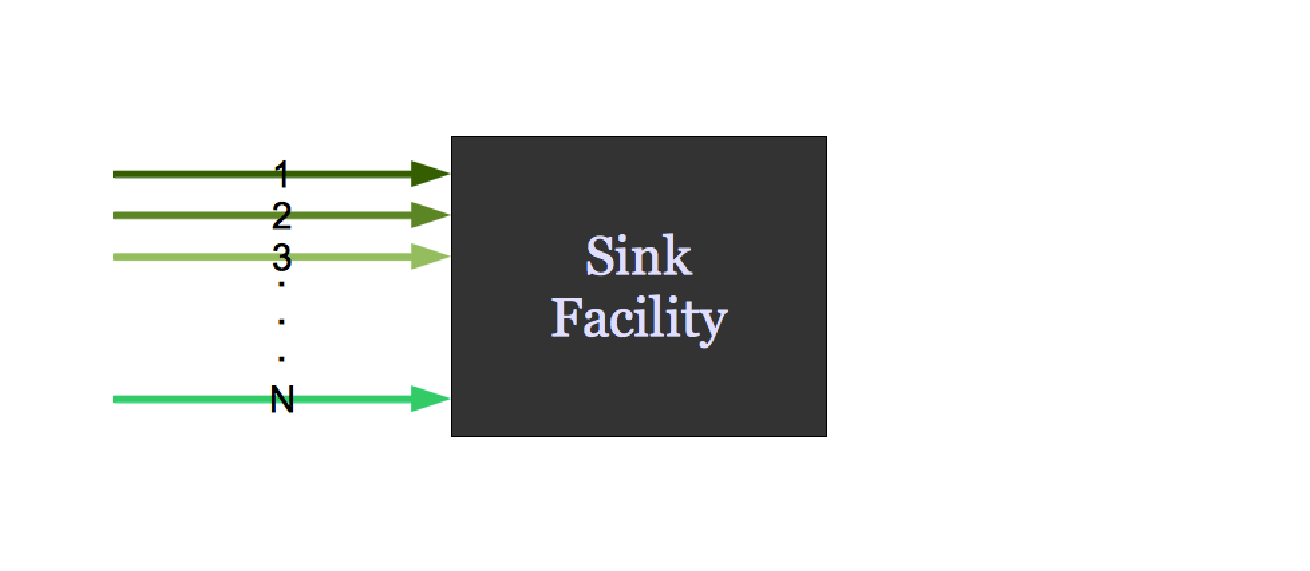
\includegraphics[width=0.7\columnwidth]{./images/sinkfacility.eps}
  \end{center}
  \caption{\footnotesize{The Cyder repository model has the same interface with the simulation 
  as does a sink facility. It receives materials according to some capacity. The 
  heat-limited capacity of the repository will be reassessed for new waste 
  streams offered to the repository.}}
  \label{fig:cydersink}
\end{figure}

\subsubsection{Specific Temperature Change Method}
Introduced by Radel, Wilson et. al., the Specific Temperature Change method uses 
a linear approximation to arrive at the thermal loading density limit.  
When the thermal time constant of the rock is much shorter than the waste form 
decay package, the change in package wall temperature can be described by 

\begin{align}
\Delta T_1 &= q(t_0)\rho_{limit}C'
\intertext{where}
\Delta T_1 &= T_{lim} - T_{amb} \nonumber\\
T_{lim} &= \mbox{ Temperature limit }[^{\circ}C]\nonumber\\
T_{amb} &= \mbox{ Ambient rock temperature }[^{\circ}C]\nonumber
q(t_0) &= \mbox{ Heat at the inital time} 
\rho_{limit} &= \frac{C_1}{Q_1}\nonumber\\
C' &= \mbox{ Thermal constant }[-]\nonumber\\
\Delta T &= T_{lim}-T_{amb}[^{\circ}C]\nonumber\\
\end{align}


\begin{figure}[htp!]
\begin{center}
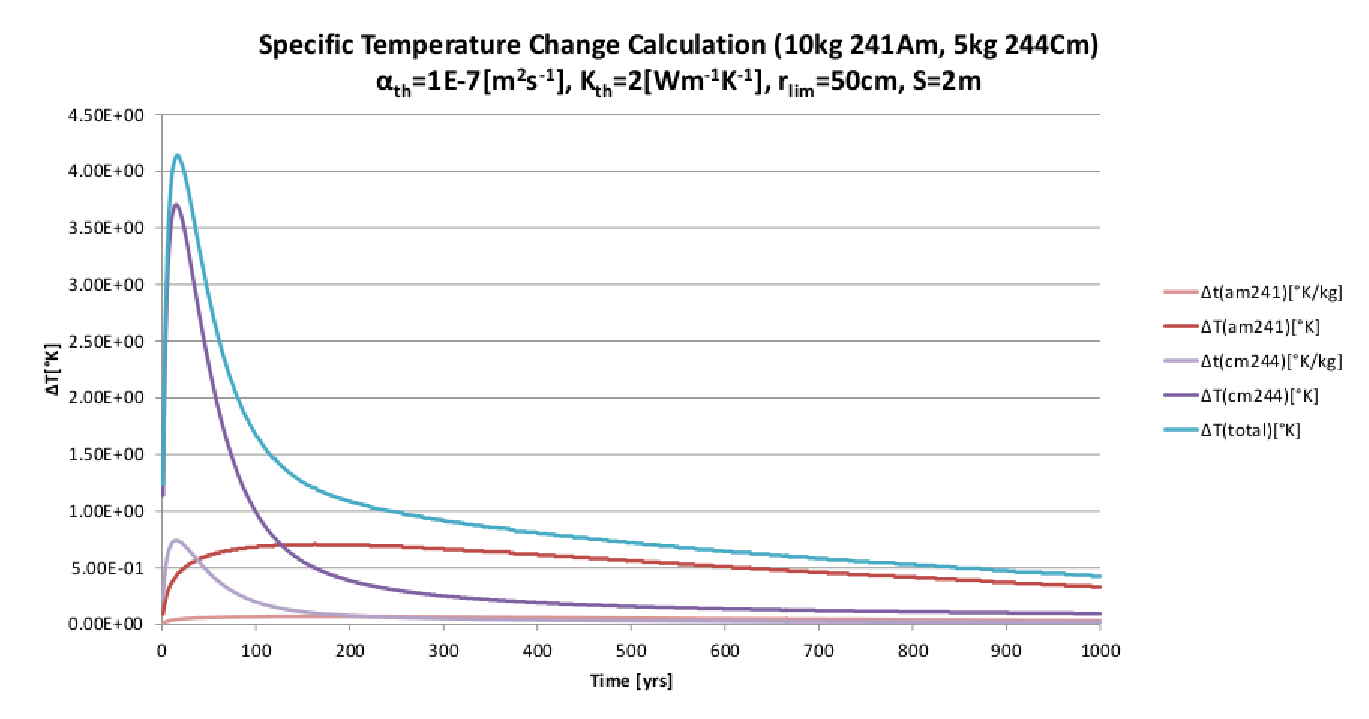
\includegraphics[width=0.8\columnwidth]{images/fakeArbitraryWF.eps}
\end{center}
\caption{\footnotesize{As a demonstration of the calculation procedure, the specific 
temperature change curves, $\Delta t$, are calculated for heat contributing 
isotopes at a 
specified repository spacing, $s$, heat limit radius, $r_{lim}$, and thermal paramters 
$\alpha_{th}$ and $K_{th}$. The total temperature change is the sum of the 
mass scaled curves $\Delta T$.}}
\label{fig:fakeArbitraryWF}
\end{figure}

Repeated runs of a detailed analytic model have given a dataset that 
facilitates estimation of thermal loading capacity for a range of thermal 
diffusitivities, conductivities, and repository layouts.
\begin{table}[ht!]
\centering
\footnotesize{
\begin{tabular}{|l|l|l|r|}
\multicolumn{4}{c}{\textbf{Thermal Cases}}\\
\hline
\textbf{Parameter} & \textbf{Symbol} & \textbf{Units} & \textbf{Value Range} \\
\hline
Diffusivity & $\alpha_{th}$ & $[m^2\cdot s^{-1}]$ & $1.0\times10^{-7}-3.0\times10^{-6}$\\
\hline
Conductivity & $K_{th}$     & $[W\cdot m^{-1} \cdot K^{-1}]$ & $0.1 - 4.5$ \\
\hline
Spacing & $S$ & $[m]$ & 2, 5, 10, 15, 20, 25, 50 \\
\hline
Radius & $r_{lim}$ & $[m]$ & 0.1, 0.25, 0.5, 1, 2, 5 \\
\hline
Isotope & $i$ & $[-]$ & $^{241,243}Am,$  \\
        & & & $^{242,243,244,245,246}Cm,$  \\
        & & & $^{238,240,241,242}Pu$  \\
        & & & $^{134,135,137}Cs$  \\
        & & & $^{90}Sr$  \\
\hline
\end{tabular}
\caption{A thermal reference dataset of \gls{STC} values as a function of each of these parameters was generated by repeated parameterized runs of the LLNL 
MathCAD model\cite{greenberg_application_2012, greenberg_investigations_2012}.}
\label{tab:thermal_cases}
}
\end{table}



\subsubsection{Supporting Thermal Response Dataset}
To support this calculation in Cyder, a reference data set of temperature change 
curves was calculated. Repeated runs of a detailed analytic model over the range of values in Table 
\ref{tab:thermal_cases} determined \gls{STC} values over a range of thermal 
heat limit radii, $r_{lim}$, thermal diffusivity values, $\alpha_{th}$,
thermal conductivity values, $K_{th}$ and waste package spacings, $S$. Linear 
interpolation across the discrete parameter space provides a simple thermal 
reference dataset for use in Cyder.

\begin{table}[ht!]
\centering
\footnotesize{
\begin{tabular}{|l|l|l|r|}
\multicolumn{4}{c}{\textbf{Thermal Cases}}\\
\hline
\textbf{Parameter} & \textbf{Symbol} & \textbf{Units} & \textbf{Value Range} \\
\hline
Diffusivity & $\alpha_{th}$ & $[m^2\cdot s^{-1}]$ & $1.0\times10^{-7}-3.0\times10^{-6}$\\
\hline
Conductivity & $K_{th}$     & $[W\cdot m^{-1} \cdot K^{-1}]$ & $0.1 - 4.5$ \\
\hline
Spacing & $S$ & $[m]$ & 2, 5, 10, 15, 20, 25, 50 \\
\hline
Radius & $r_{lim}$ & $[m]$ & 0.1, 0.25, 0.5, 1, 2, 5 \\
\hline
Isotope & $i$ & $[-]$ & $^{241,243}Am,$  \\
        & & & $^{242,243,244,245,246}Cm,$  \\
        & & & $^{238,240,241,242}Pu$  \\
        & & & $^{134,135,137}Cs$  \\
        & & & $^{90}Sr$  \\
\hline
\end{tabular}
\caption{A thermal reference dataset of \gls{STC} values as a function of each of these parameters was generated by repeated parameterized runs of the LLNL 
MathCAD model\cite{greenberg_application_2012, greenberg_investigations_2012}.}
\label{tab:thermal_cases}
}
\end{table}



The analytic model used to populate the reference dataset was created at 
\gls{LLNL} for the \gls{UFD} campaign. In this tool, heat limited thermal 
response is calculated analytically for each geology, for many waste package 
loading densities, and for many fuel cycle options \cite{hardin_generic_2011, 
greenberg_investigations_2012, greenberg_application_2012}. It employs an 
analytic model from Carslaw and Jaeger and is implemented in MathCAD 
\cite{carslaw_conduction_1959, ptc_mathcad_2010}.  The integral solver in the 
MathCAD toolset is the primary calculation engine for the analytic MathCAD 
thermal model, which relies on superposition of point, finite-line, and line 
source integral solutions.  

%The transient state of the temperature at the calculation radius is found with a convolution of the transient far field solution with the steady state near field solution.  The process is then iterated with a one year resolution in order to arrive at a temperature evolution over the lifetime of the repository. 
%
%In a two dimensional grid of waste packages, the central package is represented by the finite line solution

Figure \ref{fig:CmScaling} demonstrates the scaling of an STC curve according to 
equation \eqref{STC} to represent the heat from $25.9g$ of initial $^{242}Cm$ using 
the reference data set. 

\begin{figure}[h!]
\begin{center}
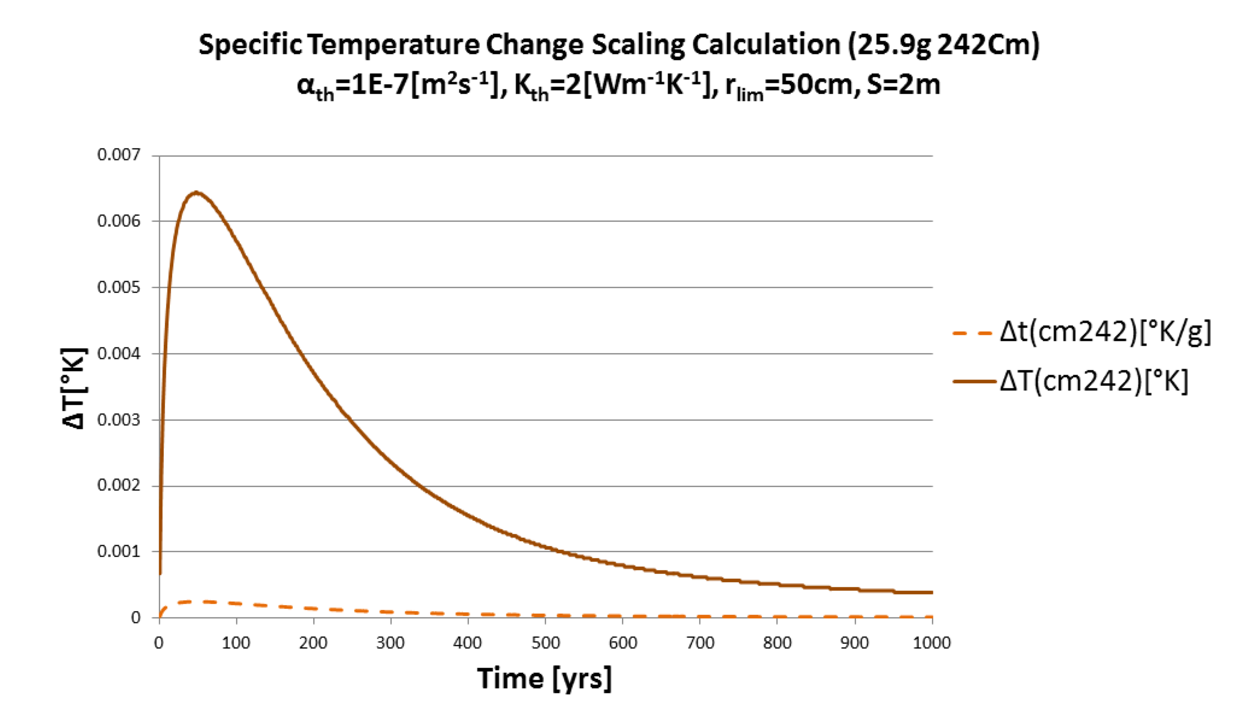
\includegraphics[width=\columnwidth]{images/CmScaling.eps}
\end{center}
\caption{As a demonstration of the calculation procedure, the temperature change 
  curve for one initial gram of $^{242}Cm$ and is scaled to represent $25.9g$, 
  approximately the $^{242}Cm$ inventory per MTHM in 51GWd burnup UOX PWR fuel. }
\label{fig:CmScaling}
\end{figure}


The supporting database was limited to  high heat contributing isotopes, $H$, 
such that the superposition in equation \eqref{superposition} becomes 

\begin{align}
\Delta T (r_{lim},S,K_{th},\alpha_{th})&\sim \sum_{i\in H} m_i \Delta t_i(r_{lim},S,K_{th},\alpha_{th})
\label{superposition_approx}
\intertext{where}
H &= \mbox{ set of high heat isotopes }[-]\nonumber\\
S &= \mbox{ uniform waste package spacing } [m]\nonumber\\
K_{th} &= \mbox{ thermal conductivity } [W\cdot m^{-1}\cdot K^{-1}]\nonumber\\
\alpha_{th} &= \mbox{ thermal diffusivity } [m^2\cdot s^{-1}]\nonumber\\
\end{align}

The use of this superposition is demonstrated in Figure 
\ref{fig:CmSuperposition}.

\begin{figure}[ht!]
\begin{center}
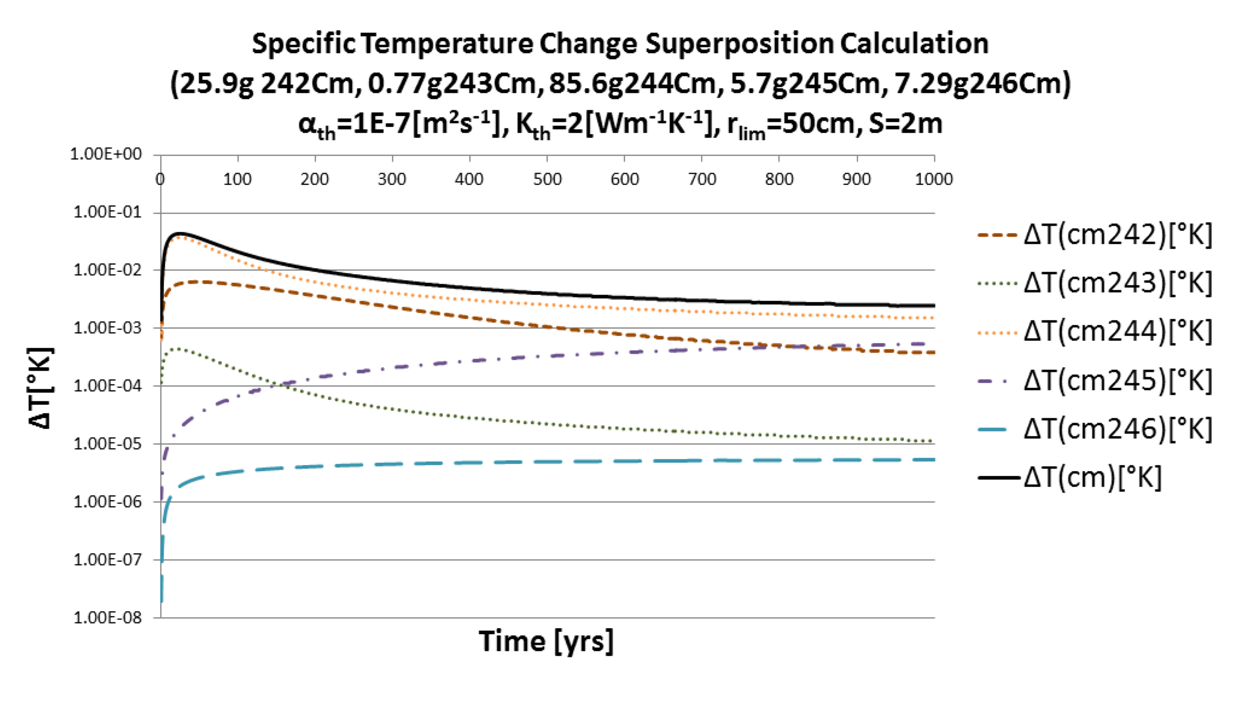
\includegraphics[width=\columnwidth]{images/CmSuperposition.eps}
\end{center}
\caption{As a demonstration of the calculation procedure, scaled temperature change 
  curves for two isotopes are superimposed to achieve a total temperature 
change (note log scale).}
\label{fig:CmSuperposition}
\end{figure}

%\begin{align}
%  T_{line}(t,x,y,z) &= \frac{1}{8\pi K_{th}} 
%  \bigintsss_0^t\!\frac{q_L(t')}{t-t'}e^{ \frac{-\left(x^2 + z^2\right)}{4\alpha 
%  (t-t')} }\nonumber\\ &\cdot\left[ \erf{\left[ \frac{1}{2} \frac{\left( y + 
%  \frac{L}{2} \right)}{\sqrt{\alpha(t-t')}}  \right]} - \erf{\left[ \frac{1}{2} 
%  \frac{\left( y - \frac{L}{2} \right)}{\sqrt{\alpha(t-t')}}  \right]} 
%  \right]\,\mathrm{dt'},
%  \label{line}
%  \intertext{adjacent packages within the central tunnel are represented by the 
%  point source solution }
%  T_{point}(t,r) &= 
%  \frac{1}{8K_{th}\sqrt{\alpha}\pi^{\frac{3}{2}}}\bigintsss_0^{-t}\!\frac{q(t')}{(t-t')^{\frac{3}{2}}}e^{\frac{-r^2}{4\alpha(t-t')}}\,\mathrm{dt'},
%  \label{point}
%  \intertext{and adjacent disposal tunnels are represented by infinite line 
%  source solutions}
%  T_{\infty line}(t,x,z) &= \frac{1}{4\pi K_{th}} 
%  \bigintsss_0^t\!\frac{q_L(t')}{t-t'}e^{ \frac{-\left(x^2 + z^2\right)}{4\alpha 
%  (t-t')} }
%  \intertext{in infinite homogeneous media, where}
%  \label{infline}
%  \alpha &= ~~\mbox{thermal diffusivity } [m^2\cdot s^{-1}]\nonumber\\
%  q(t) &= ~~\mbox{point heat source} [W]\nonumber\\
%  \intertext{and}
%  q_L(t) &= ~~\mbox{linear heat source} [W\cdot m^{-1}]\nonumber
%\end{align}
%Superimposed point and line source solutions allow for a notion of the 
%repository layout to be modeled in the host rock.

